The selection of suitable sequences for the subject test is based on technical considerations and content.

\subsubsection{Preconsiderations}
The number of public video databases with royalty free \textit{UHD-1} and 4k video material is limited. They differ in content (scenario, field size, camera movement, illumination condition) and in technical aspects (resolution, frame rate, bitrate and color bit depth).
To obtain reference video files for the subjective test, parts of the \textit{UHD-1} content from the databases are used (also called source video files).
For our test we want to have a large variety between the reference video files to evoke different encoding properties.
All the reference videos should have a duration of 10 seconds as they represent a single \textit{HAS}-segment and should contain no hard cuts.
To avoid the influence of judder, the smallest permitted frame rate of the source videos is 50 frames per second (fps). Furthermore the smallest resolution considered to be 3840x2160. Moreover the frame rate of the reference video files is being adapted to consistent 50 fps and the resolution to 3840x2160 pixels.

\subsubsection{Dataset Preparation}
For obtaining a good variety of video sequences three databases are used: The Harmonic \cite{web:harmonic} which contains 18 different video files, Cable Labs \cite{web:cablelabs} with 9 relevant \textit{UHD-1} contents and the Blender Foundation \cite{web:bbb} for receiving the cartoon Big Buck Bunny. They  are partial under the creative commence license and all of them are available in the \textit{ProRes} format, except of Big Buck Bunny where the \textit{UHD-1} video content can be downloaded only as a compressed video file, however there also exist high quality PNGs for all the frames of the cartoon. In order to generate a high quality reference video with the frames of Big Buck Bunny, an automatisation script is used to find a sequence with a duration of 10 seconds, to download the respective images and to encode them as a video file.
The main challenge is finding periods of video without cuts that are 10 seconds or longer, as only a few of those are available, which is also a limiting factor for the content diversity.

One problem of the video sequences from the database is that even if they have high bitrates and are stored as \textit{ProRes}, no assumptions can be made on the visual quality of the material. It would be preferred to have the source videos available in RAW format as this assures no loss of information and no previous processing.
For this reason a preselection with a system able to play UHD content in \textit{ProRes} with high bitrates and connected to a 4k screen, was applied.
The remaining reference videos are 6 source clips, each with a duration of 10 seconds. All the files exhibit a minimum resolution of 3840x2160 pixels and are stored in \textit{ProRes}. Because this format is a 10 bit codec only \cite{web:ProRes}, the original color depth of each video file can not be determined.
Further specific information about the reference videos are shown in Table \ref{tab:Specifications}, e.g. Air Show, a video from the Harmonic Database, available with 59.94 fps and a bitrate of 1703 Mbit/s. For obtaining the reference video with a duration of 10 seconds the extraction starts at the 48.5 second of the source video file.

\begin{table}[hbt!]
	\renewcommand{\arraystretch}{1.3}
	\centering
	\caption{Meta data of the video files. The timestamps are the start positions of the extraction of 10 second sequences from the source files, where mm stands for minutes, ss for seconds and ms for milliseconds respectively. Further shortcuts: H = Harmonic, B = Blender Foundation, C = Cable Labs}
	\label{tab:Specifications}
	\begin{tabular}{lcccc}
		%\cline{2-6}
		\toprule
		Sequence Name       & Frame Rate & Bit rate & Timestamps & Source\\
		& fps  	   & Mbits/s    & mm:ss.ms   & \\
		\midrule
		Air Show            & 59.94    & 1703 & 00:48.500  &   H  \\
		Big Buck Bunny      & 60       & 2304 & 05:47.000  &   B  \\
		Fjord               & 50       & 1469 & 00:21.000  &   H  \\
		Moment of Intensity & 59.94    & 1822 & 02:16.000  &   C \\
		Snow Monkeys        & 59.94    & 1750 & 00:17.000  &   H  \\
		Streets of India    & 50       & 2094 & 00:00.000  &   H  \\
		\bottomrule
	\end{tabular}
\end{table}

They contain a wide range of high-level features (animation, camera motion, people, water) and low-level characteristics (brightness, contrast, texture, motion, color variance, sharpness) as can be seen in Figure \ref{fig:OverviewReferenceSequences}.

\begin{figure}[hbt!]
	\begin{center}
		%

		\subfigure[Air Show]{%
			\label{fig:airshow}
			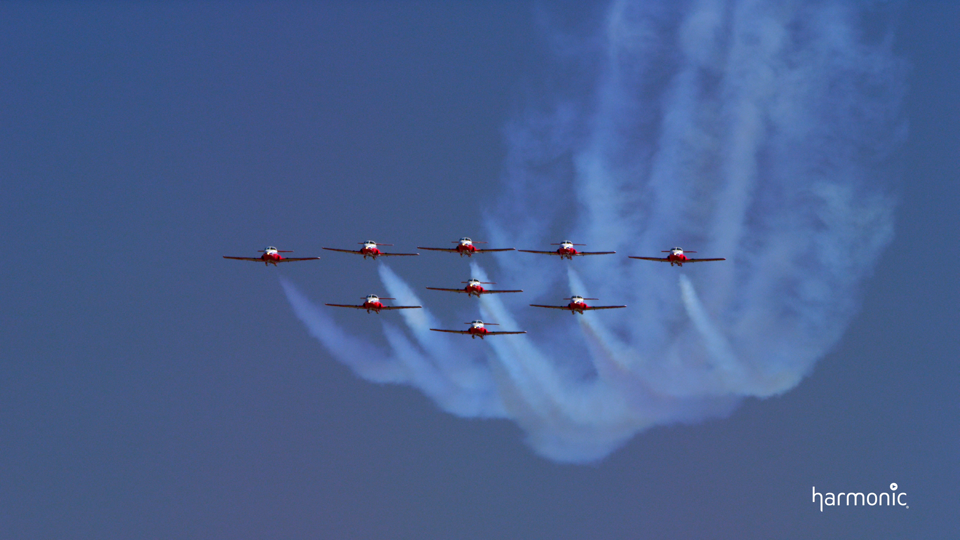
\includegraphics[width=0.2\textwidth]{images/AirShow}
		}%
		\subfigure[Big Buck Bunny]{%
			\label{fig:bbb}
			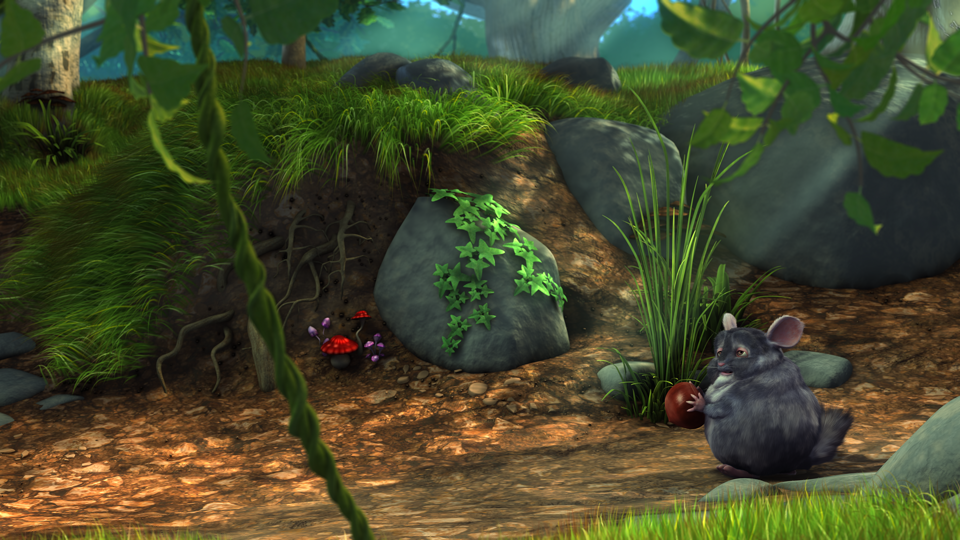
\includegraphics[width=0.2\textwidth]{images/Bbb}
		}\\ %  ------- End of the first row ----------------------%
		\subfigure[Fjord]{%
			\label{fig:Fjord}
			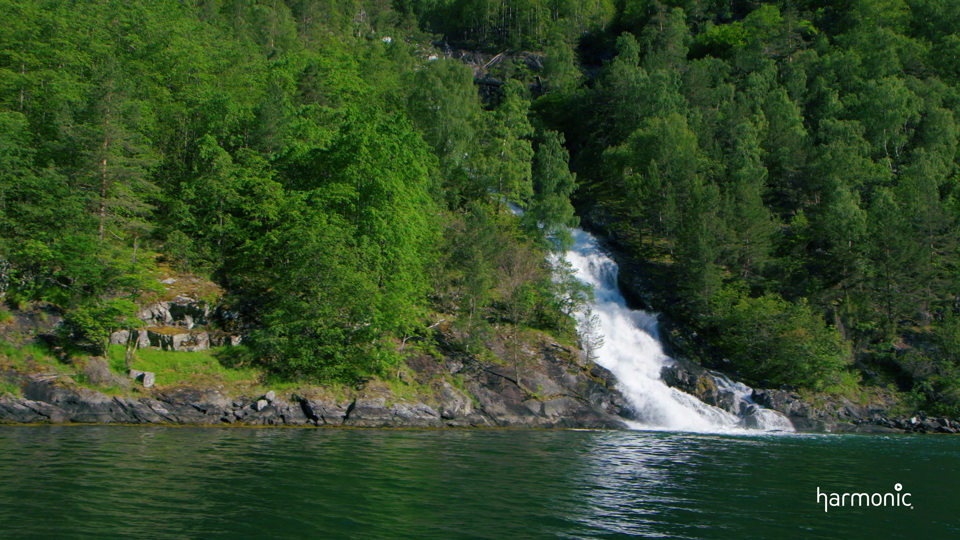
\includegraphics[width=0.2\textwidth]{images/Fjord}
		}%
		\subfigure[Moment of Intensity]{%
			\label{fig:MomentOfIntensity}
			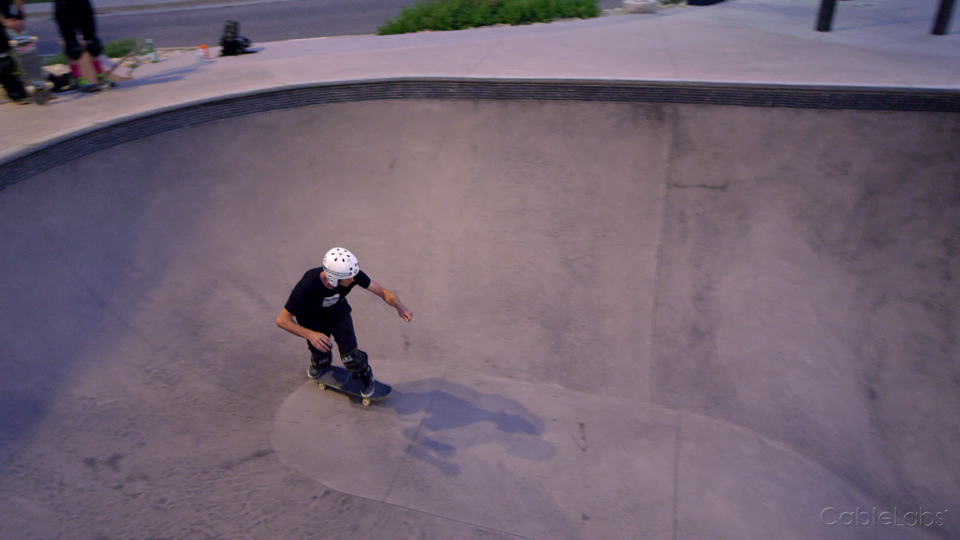
\includegraphics[width=0.2\textwidth]{images/MomentOfIntensity}
		}\\ %  ------- End of the second row ----------------------%		
		\subfigure[Snow Monkeys]{%
			\label{fig:SnowMonkeys}
			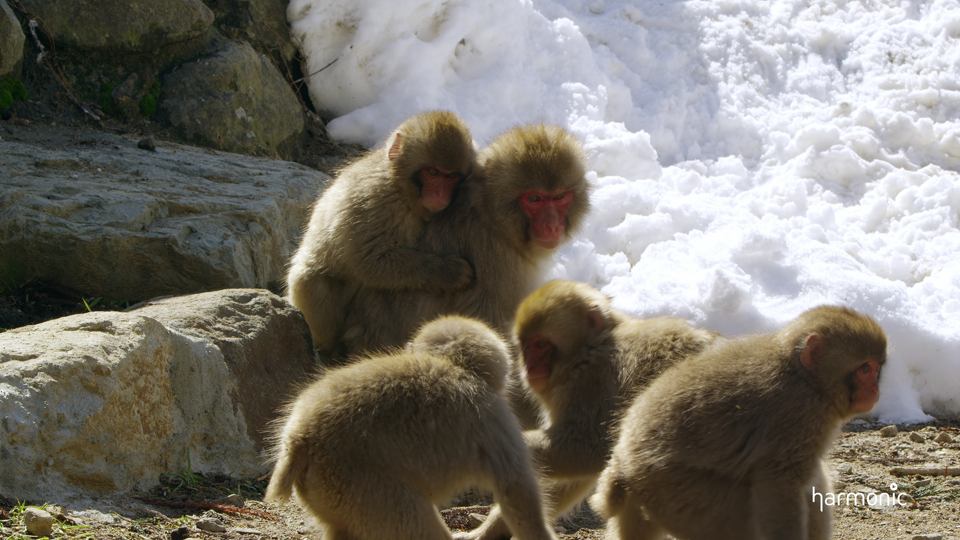
\includegraphics[width=0.2\textwidth]{images/SnowMonkeys}
		}%
		\subfigure[Streets of India]{%
			\label{fig:StreetsOfIndia}
			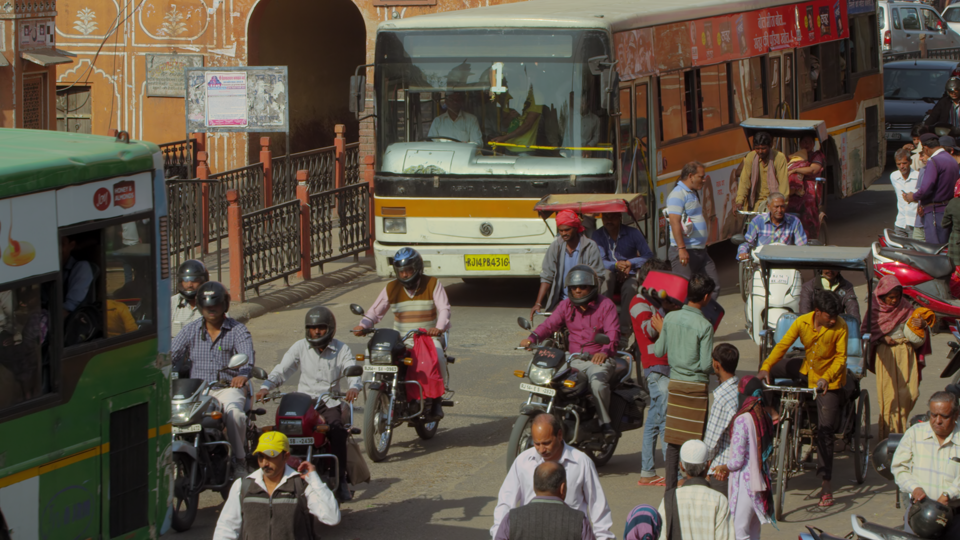
\includegraphics[width=0.2\textwidth]{images/StreetsOfIndia}
		}%
		%
	\end{center}
	\caption{%
		Selection of frames contained in the reference videos to show the variety of the content.
	}%
	\label{fig:OverviewReferenceSequences}
\end{figure}

\begin{figure}[hbt!]
	\centering
	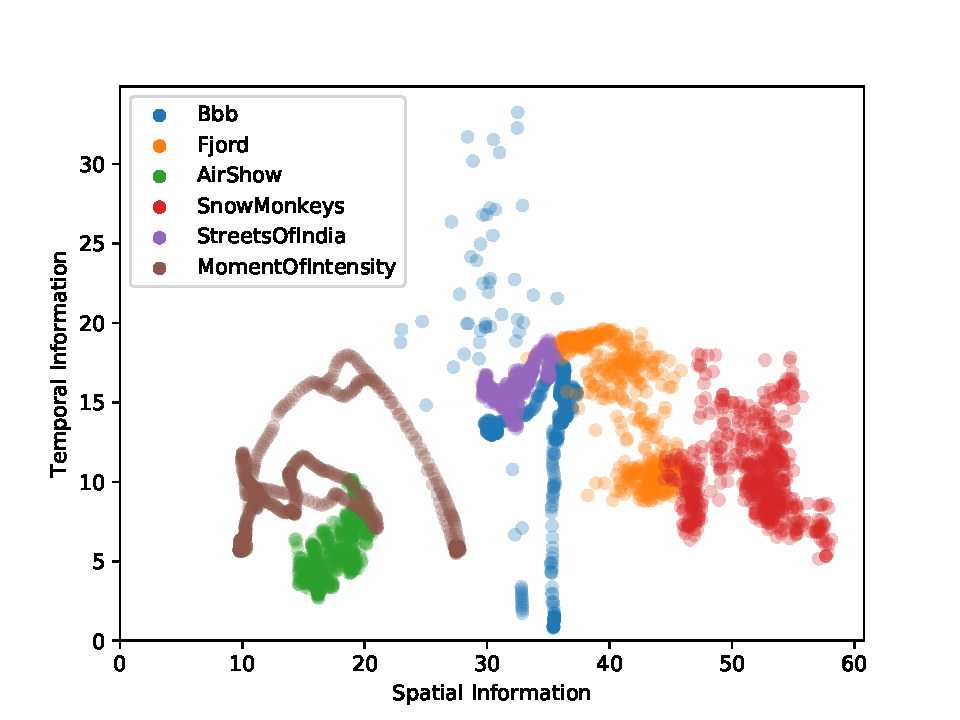
\includegraphics[width=3.5in]{SITI}
	\caption{Spatial and temporal information of the reference video files. Each dot represents one frame. In areas with high densities the color is stronger.}
	\label{fig:SITI}
\end{figure}

We further analyzed the spatial and temporal changes between the frames of each reference video with SITI \cite{web:SITI}, a command-line-based tool that refers to ITU-T P.910. The results can be seen in Figure \ref{fig:SITI}.
The spatial information is derived as the maximum standard derivation of the results of a sobel filter applied on each frame. Furthermore the temporal information is the maximum standard derivation of the motion difference between two frames at the same location in space.
As expected, the Air Show sequence includes the smallest spatial and temporal changes in comparison with the other reference videos due to the only slightly changing, low complexity scenario. In contrast to that the Big Buck Bunny sequence shows a large range of temporal differences because of camera movement, while the Snow Monkeys sequence has the highest spatial information due to fine structures and details.

The following section goes into detail on how the chosen sequences are encoded for the subjective test.


